\documentclass[12pt]{article}
\usepackage[utf8]{inputenc}
\usepackage{graphicx}
\graphicspath{ {/home/Arif Khan/Pictures/} }
\usepackage{ragged2e}
\usepackage{geometry}
\usepackage{amsmath}
\usepackage{amssymb}
\usepackage{listings}
\usepackage{tikz}
\usepackage{url}
\usepackage{hyperref}
\usetikzlibrary{shapes.geometric, arrows}
\renewcommand{\baselinestretch}{1.5}

\begin{document}

\begin{center}
\textbf{Assignment-8 \\
\vspace{5mm}
ELP - 718 Telecom Software Laboratory \\
\vspace{2mm}
Arif Khan \\
2018JTM2242 \\
2018-2020} \\
\vspace{10mm}
A report presented for the assignment on Python Basic and Github\\
\vspace{30mm}
\includegraphics[scale=0.5]{/home/arifkhan/Desktop/iitlogo.jpeg} \\
\vspace{10mm}
Bharti School Of \\
Telecommunication Technology and Management \\
IIT Delhi \\
India \\
September 27, 2018
\newpage
\tableofcontents
\newpage

\end{center}
\section{Problem Statement-1} 
IIT Delhi, has just got the strongest computer. The professors in charge wants to check the computational capacity of the computer. So, they decided to create the problem which is to be given as an assignment to students. Can you help the professor to check the computation capability of the computer?

A valid cross is defined here as the two regions (horizontal and vertical) of equal lengths crossing over each other. These lengths must be odd, and the middle cell of its horizontal region must cross the middle cell of its vertical region.\\
Find the two largest valid crosses that can be drawn on smart cells in the grid, and return two integers denoting the dimension of the each of the two largest valid crosses. In the above diagrams, our largest crosses have dimension of 1,  5 and 9 respectively .
\begin{itemize}
\item  Note: The two crosses cannot overlap, and the dimensions of each of the valid crosses should be maximal.

\end{itemize}




\subsection{Program Structure}
\begin{lstlisting}

\end{lstlisting}


\subsection{Difficulties}
\begin{itemize}
\item We faced difficulties during overcome the problem of overlap of crosses. 
\item We faced difficulties during formation of cross.
\item Faced problem to remove error .
\item We faced problems during execute the code.

\end{itemize}
\subsection{Algorithm}
\begin{itemize}
\item Take N number of sample   strings to formed crosses.
\item Identify the character in each string whether it is DULL(D) or SMART(S).
\item On the basis  of "S" we create crosses.
\item Find largest and smaller dimensions crosses.
\item Print the Dimensions in Decreases order.

\end{itemize}




\subsection{Flowchart}
%\begin{figure}[h]

   
\begin{center}
          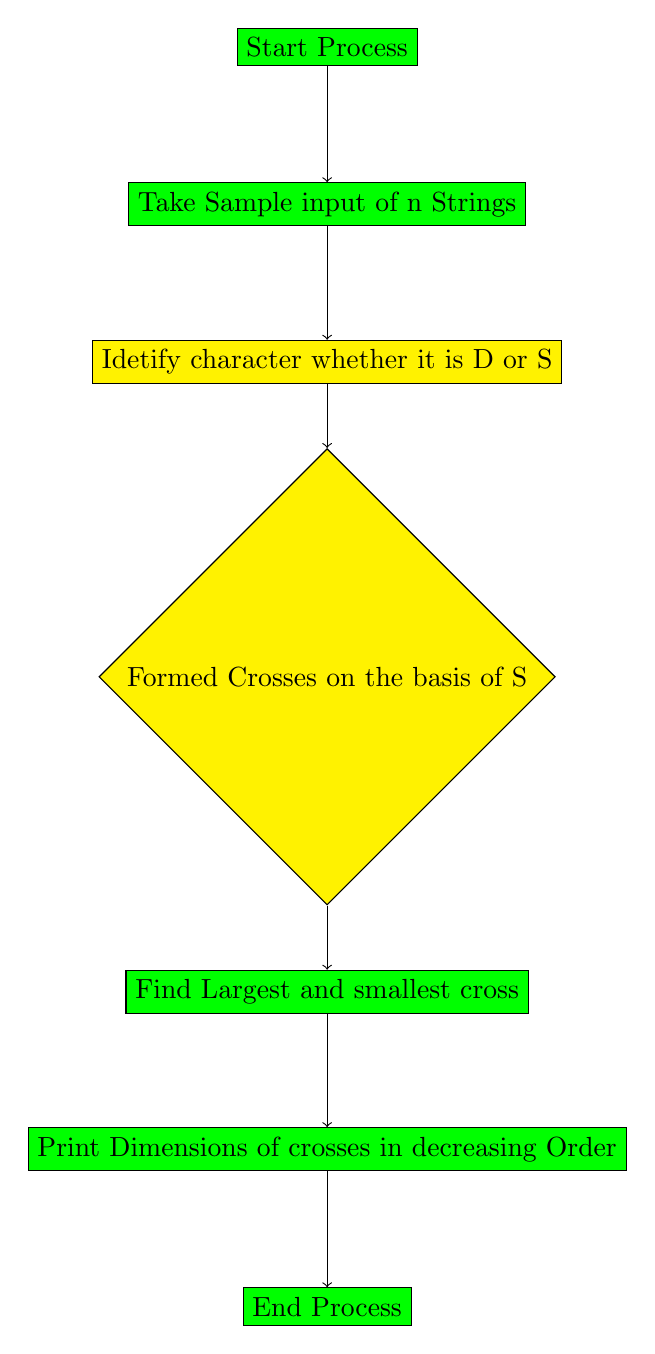
\begin{tikzpicture}
            \node[draw,shape= rectangle,fill=green,scale=1](n1)at(0,0){Start Process};
            \node[draw,shape=rectangle,fill=green,scale=1](n2)at (0,-2){Take Sample input of n Strings };     
            \node[draw,shape=rectangle,fill=yellow,scale=1](n3)at (0,-4){Idetify character whether it is D or S};
                  
             %\node[draw,shape=rectangle,fill=yellow,scale=1](n4)at (0,-6){Find the number of all emoticons in text messages };
       
            \node[draw,shape=diamond,fill=yellow,scale=1](n4)at (0,-8){Formed Crosses on the basis of S  };
            \node[draw,shape= rectangle, fill=green,scale=1](n5)at (0,-12){Find Largest and smallest cross};
            
            \node[draw,shape= rectangle, fill=green,scale=1](n6)at (0,-14){Print Dimensions of crosses in decreasing Order};
                      \node[draw,shape= rectangle, fill=green,scale=1](n7)at (0,-16){End Process};
              % \node[draw,shape= rectangle, fill=green,scale=1](n7)at (0,-17){End Program};
                                
       %\node[draw,shape= rectangle, fill=white,scale=1](n8)at (8,-12){YES};
           
            
            %\node[shape=rectangle,fill=white,scale=1](n6)at (.8,-7.8){YES};
           % \node[draw,fill=red](n3)at(10,0){Rx};
    
            \draw[->](n1)to[](n2);
            \draw[->](n2)to[](n3);
            \draw[->](n3)to[](n4);
             \draw[->](n4)to[](n5);
              \draw[->](n5)to[](n6);
               \draw[->](n6)to[](n7);
              
                %\draw[->](n6)to [](n8);
                % \draw[->](n8)to [](n3);
                
               %\draw[->](n6)to[](n7); 
                
           % draw[->](n6)to[](n7);
           \end{tikzpicture}
            %\caption{Record Of Employee}
           \end{center}
     %  \end{figure}
\newpage


\subsection{Input Format}
Input is given through a text file.
\subsection{Output Format}
Output is taken through user commmand line argument.

%\includegraphics[scale=0.5]{/home/arifkhan/Desktop/ps1.png} 

\section{Problem Statement-2}
After, getting mix results of valid crosses, professors decided to test the computation abilities on one more problem. This time professors wanted to test the decryption capabilities of the computer.\\
Encryption of  a message requires three keys, k1, k2, and k3. The 26 letters of English and underscore are divided in three groups,  [a-i] form one group, [j-r] a second group, and everything else ([s-z] and underscore) the third group. Within each group the letters are rotated left by ki positions in the message. Each group is rotated independently of the other two. Decrypting the message means doing a right rotation by ki positions within each group.



\subsection{Program Structure}
\begin{lstlisting}
> ###### this is the second .py file ###########
>
> ####### write your code here ##########
> #rotate function
> def rotate(lst,x):
>     copy = list(lst)
>     for i in range(len(lst)):
>         if x<0:
>             lst[i+x] = copy[i]
>         else:
>             lst[i] = copy[i-x]
>
>
> #Create 3 groups
> g1="abcdefghi"
> g2="jklmnopqr"
> g3="stuvwxyz_"
>
> c1 =[]
> c2 =[]
> c3 =[]
> index1=[]
> index2=[]
> index3=[]
>
> #get key vakue from user
> k1,k2,k3 = list(map(int,input().split()))
>
> #get string
> msg = input()
> msg_list = list(msg)
> print(msg_list)
>
> #now compair g1 in string and copy similaar char into s1
> for i in range(0,len(msg)):
>     if msg_list[i] in g1:
>         c1.append(msg_list[i])
>         index1.append(i)
>
>     elif msg_list[i] in g2:
>         c2.append(msg_list[i])
>         index2.append(i)
>     elif msg_list[i] in g3:
>         c3.append(msg_list[i])
>         index3.append(i)
>
>
>
> #rotate c1,c2,c3
> rotate(c1,k1)
> rotate(c2,k2)
> rotate(c3,k3)
>
>
>
> #get decrypted msg
> p=q=r=0
> for i in range(0,len(msg)+1):
>     if i in index1:
>         msg_list[i]=c1[p]
>         p+=1
>     elif i in index2:
>         msg_list[i]=c2[q]
>         q+=1
>     elif i in index3:
>         msg_list[i]=c3[r]
>         r+=1
>
> print(msg_list)
>
> for i in msg_list[:]:
>     print (i, end ='')
>
> print(\n)


\end{lstlisting}


\subsection{Algorithm}
\begin{itemize}
\item Take N number of sample strings.
\item  We  divide all alphabets in K1,K2 AND K3 keys.
\item For encryption  we rotate characters  left corresponding to Key.
\item For Decryption  we rotate characters  Right corresponding to Key.

\item Print the Decrypted string.
 
\end{itemize}






\subsection{Input Format}


\subsection{Output Format}
%\includegraphics[scale=0.5]{/home/arifkhan/Desktop/ps2.png} 

\subsection{Difficulties}
\begin{itemize}
\item We faced difficulties during overcome the problem of repetation of character. 
\item We faced difficulties during Decryption and Encryption  of strings.
\item Faced problem to remove error .
\item We faced problems during execute the code.
\end{itemize}

\subsection{Flowchart}

  \begin{center}
          \begin{tikzpicture}
            \node[draw,shape= rectangle,fill=green,scale=1](n1)at(0,0){Start  Process};
            \node[draw,shape=rectangle,fill=green,scale=1](n2)at (0,-3){Take a String as Sample };     
            \node[draw,shape=rectangle,fill=yellow,scale=1](n3)at (0,-5){Encryption the Message string by Left rotating };
                  
            
       
            \node[draw,shape=diamond,fill=yellow,scale=.75](n4)at (0,-10){Decryption of message string by Right ritating};
            
              \node[draw,shape= rectangle, fill=green,scale=1](n5)at (0,-16){Print the Decrypted string };
              
      
      \node[draw,shape= rectangle, fill=green,scale=1](n6 )at (0,-18){End Process};        
      
      
      %\node[draw,shape= rectangle, fill=white,scale=1](n8)at (8,-12){YES};
           
            
            %\node[shape=rectangle,fill=white,scale=1](n6)at (.8,-7.8){YES};
           % \node[draw,fill=red](n3)at(10,0){Rx};
    
            \draw[->](n1)to[](n2);
             \draw[->](n2)to[](n3);
              \draw[->](n3)to[](n4);
               \draw[->](n4)to[](n5);
                \draw[->](n5)to[](n6);
               %\draw[->](n6)to[](n7);
              
                %\draw[->](n7)to [](n8);
                % \draw[->](n8)to [](n3);
                
               %\draw[->](n6)to[](n7); 
                
           % draw[->](n6)to[](n7);
           \end{tikzpicture}
            %\caption{Record Of Employee}
           \end{center}
     %  \end{figure}     


\nocite{*}
\bibliographystyle{plain}
\bibliography{jtm182242.bib}

\end{document}